% !TeX program = pdflatex
\documentclass[tikz,border=8pt]{standalone}
\usepackage{pgfplots}\pgfplotsset{compat=1.16}
\definecolor{FigureBlue}{HTML}{2563EB}\definecolor{FigureOrange}{HTML}{EA580C}
\begin{document}
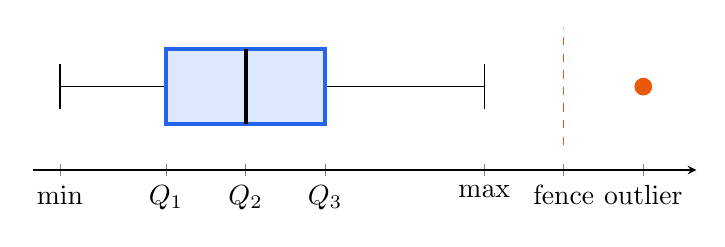
\begin{tikzpicture}
\begin{axis}[width=10cm,height=3.7cm,axis y line=none,axis x line=middle,xmin=-.5,xmax=12,ymin=0,ymax=2,xtick={0,2,3.5,5,8,9.5,11},xticklabels={min,$Q_1$,$Q_2$,$Q_3$,max,fence,outlier},ytick=\empty,clip=false]
  \addplot[only marks,mark=|,mark size=8pt] coordinates {(0,1)(8,1)};
  \draw (axis cs:0,1)--(axis cs:2,1) (axis cs:5,1)--(axis cs:8,1);
  \draw[FigureBlue,fill=FigureBlue!15,line width=1.2pt] (axis cs:2,.55) rectangle (axis cs:5,1.45);
  \draw[line width=1.4pt] (axis cs:3.5,.55)--(axis cs:3.5,1.45);
  \draw[dashed,FigureOrange] (axis cs:9.5,.3)--(axis cs:9.5,1.7);
  \addplot[only marks,mark=*,mark size=3pt,FigureOrange] coordinates {(11,1)};
\end{axis}
\end{tikzpicture}
\end{document}
